\section{Study Design}
\label{sec:design}

% In this section, we describe the data collection process and 
% the overview of the collected dataset. 
In this section, we describe our study design. 
In particular, we describe research questions and 
the data collection process.

\subsection{Research Questions}
\label{sec:rqs}

To clarify the characteristics of 
the visual issue reports,
% with images and movies, 
% we executed an initial analysis 
% in our dataset. 
% Specifically, 
we addressed the following 
two research questions. 
\begin{itemize}
	\item[RQ1:] \textbf{\RQone{}}\\
	The feature to share movies on GitHub 
	is still new. 
	Hence, we suppose that using visualization 
	is not popular for developers. 
	In this RQ, we counted the number of 
	issues that use either issues or movies 
	to clarify whether using visualization 
	is popular. 
	\item[RQ2:] \textbf{\RQtwo{}}\\
	We suppose that developers use visualization 
	in particular issues. 
	For example, developers may use visualization 
	to share the way to reproduce bugs. 
	In this RQ, we clarify the differences 
	between the issues with and without 
	visualization. 
\end{itemize}


\begin{figure*}[t]
\centering
% 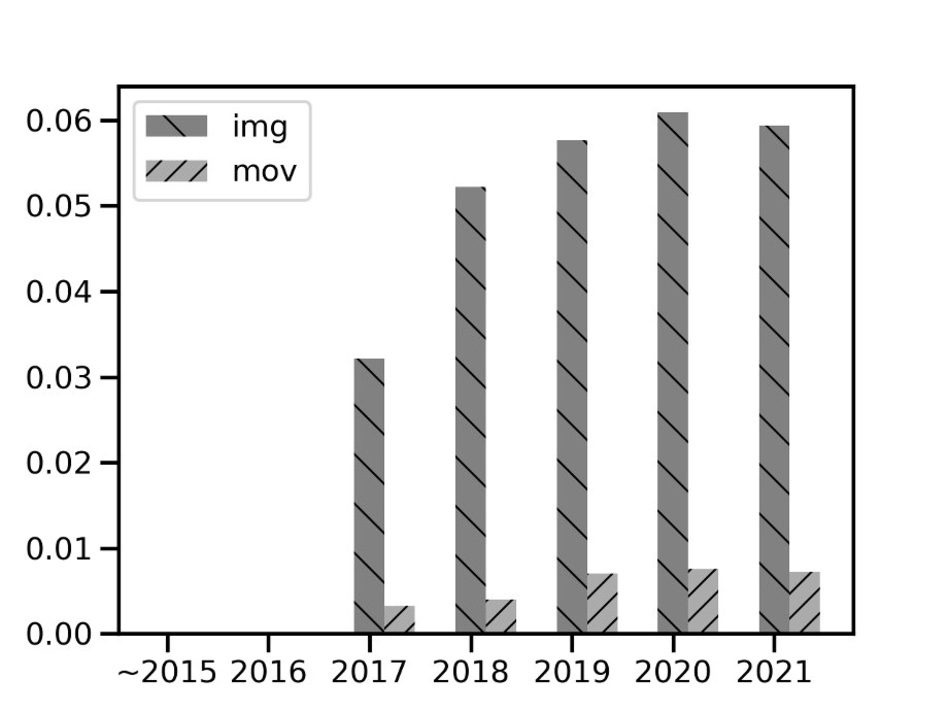
\includegraphics[width=1\linewidth]{./figures/data-category-trend.pdf}
\caption{ 
  An overview of the data collection
  }
\label{fig:data-collection-overview}
\end{figure*}


\subsection{Data Collection}
\fig{fig:data-collection-overview} shows
an overview of the data collection process.
We collected the data from the issues of 
the publicly available repositories on GitHub. 
We first select the repositories based on the following conditions:
\begin{itemize}
	\item the number of stars $\geq$ 10
	\item the number of issues $\geq$ 1
	\item the latest commit is in 2021
\end{itemize}
We used the number of stars for retrieving the repositories 
in which the owner may communicate with other developers and 
discard repositories developed by only the owner. 
In addition, we used the date of the latest commit 
because the major release of the feature is in 2021. 
Beforehand, the feature was the beta version. 
The number of the repositories that meet 
the conditions is 289,115. 
We randomly selected 4,173 repositories from them 
due to the execution time to collect issues. 
This number is less than 2\% of all repositories. 
However, the number of resolved issues 
in these repositories is already 770,656. 
We discuss the threat to validity of 
this process in \sec{sec:limitation}. 
This process was conducted from November 2021 to December 2021.


\begin{table}[t]
    \begin{center}
    \caption{The attributes we collected from the issues}
    \scalebox{0.85}[0.85]{
    \begin{tabular}{ll} 
        \toprule
        \multicolumn{1}{c}{\textbf{Attributes}} & \multicolumn{1}{c}{\textbf{Description}} \\ 
        \midrule
        $IssueResolvedTime$ & The time until the issue is resolved (day) \\
        $FirstCommentTime$ & The time until the first comment (day) \\
        $\#comments$ & The number of comments \\
        $\#chars$ & \masa{im not sure what is this} \\
        $\#imgs$ & \# of attached images when the issue is created \\
        $\#movs$ & \# of attached movies when the issue is created \\
        $\#words$ &  \masa{im not sure what is this} \\
        $IssueCreatedYear$ & The year when the issue is created \\
        \bottomrule
    \end{tabular}
    }
    \label{tab:issue-attr}
    \end{center}
\end{table}


We retrieved the attributes from the collected issues 
that are the data in the database. 
\tab{tab:issue-attr} shows the eight attributes 
retrieved from the issues. 

We used \texttt{PyGitHub}\masa{add citation} to execute GitHub API 
to retrieve the attributes from the issues. 
$IssueOpenTime$, $FirstCommentTime$,
and $IssueCreatedYear$ can be directly
retrieved by \texttt{PyGitHub}.
On the contrary,
$\#chars$, $\#imgs$, $\#movs$, and $Words$
need the conversion from the retrieved raw data.
We describe the details of the conversion. 
It should be noted that we converted the first description of 
issues into these four attribute values and 
ignore the comments and the title.
\masa{Is this description correct?}

The attached images and movies are transformed into 
URLs and put in the text of issues as the markdown format. 
The following URL is an example.

\begin{quote}
	https://user-images.githubusercontent.com/XXX.mp4
\end{quote}

\noindent{}
The part of XXX consists of alphanumeric, ``/'', and ``-''.
Hence, we prepared the regular expression for this URL and 
count the appearances of images and movies as $\#imgs$ and $\#movs$. 
The identification of images and movies is based on the extension of 
the URLs. 
Specifically, we used png, PNG, jpg, JPG, and jpeg as 
the extensions for images and 
gif, GIF, mp4, MP4, and mov as the extensions for movies.

We counted the number of characters as $\#chars$ and 
stored the words as $Words$ for all issues. 
In this process, if the description of the issue 
includes the URL, we exclude it from the description, 
and convert all issues into $\#chars$ and $Words$.
% For the issues that include the URL, we excluded them and 
% counted the number of words as $\#words$. 
% In addition, we counted the number of characters as $\#chars$. 

We noticed that some $IssueOpenTime$ values are less than zero. 
We decided that these values are invalid and the issues having 
these values are excluded from the dataset. 
In addition, to study the impact of movies and images on 
the communication in issues, 
we excluded issues that resolved less than 30 secs. 
This is because this issue resolution time is too short 
to communicate with each other. 
Specifically, we only retrieved the issues that meet 
the condition: $30\ sec \leq IssueOpenTime \leq 1\ year$.
The number of issues that meet this condition is 711,160 (92.23\%).


\begin{table}[h]
    \begin{center}
    \caption{The number of issues for each category}
    \begin{tabular}{llr}
        \toprule
         & \multicolumn{1}{c}{\textbf{Description}} & \multicolumn{1}{c}{\textbf{\#issues}} \\
        \midrule
        $Img$  & $\#imgs \geq 1$ & 33,079 (4.65\%)\\
        $Mov$  & $\#movs \geq 1$ & 3,819 (0.54\%)\\
        $None$ & Others & 674,793 (94.81\%)\\ 
        \bottomrule
    \end{tabular}
    \label{classify_result}
    \end{center}
\end{table}


We classified the issues into three categories based on 
whether they have images and movies. 
\tab{tab:issue-category} shows the number of issues for each category. 
It should be noted that issues that have both 
the images and movies are counted for both 
$Img$ and $Mov$ categories. 

% \begin{table*}[h]
    \begin{center}
    \caption{Examples of the retrieved issues with the values of the attributes}
    \begin{tabular}{c c c c c c c} 
      \toprule
      \textbf{IssueCreatedYear} &
      \textbf{ResolutionTime} &
      \textbf{Images} &
      \textbf{Videos} &
      \textbf{Comments} &
      \textbf{FirstCommentTime} &
      \textbf{DescriptionLength} \\
      \midrule
      2020 & 6.99861111 & 0 & 0 & 1 & 6.99861111 & 4430\\
      2020 & 41.9594329 & 1 & 0 & 3 & 17.7784722 & 85\\
      2020 & 43.8850579 & 0 & 0 & 2 & 0.49828704 & 56\\
      2020 & 44.0935532 & 0 & 0 & 4 & 0.91277778 & 33\\
      2020 & 0.14934028 & 0 & 0 & 8 & 0.08077546 & 244\\
      2020 & 59.5670949 & 2 & 0 & 5 & 0.39472222 & 102\\
      2020 & 74.9322569 & 0 & 0 & 0 & -          & 24\\
      \bottomrule
    \end{tabular}
    \label{tab:example-dataset}
    \end{center}
  \end{table*}

% We extract a part of the retrieved issues in \tab{tab:example-dataset}. 
% Each row corresponds to the values of the attributes of an issue. 
